% TEMPLATE for Usenix papers, specifically to meet requirements of
%  USENIX '05
% originally a template for producing IEEE-format articles using LaTeX.
%   written by Matthew Ward, CS Department, Worcester Polytechnic Institute.
% adapted by David Beazley for his excellent SWIG paper in Proceedings,
%   Tcl 96
% turned into a smartass generic template by De Clarke, with thanks to
%   both the above pioneers
% use at your own risk.  Complaints to /dev/null.  make it two column with no
% page numbering, default is 10 point

% Munged by Fred Douglis <douglis@research.att.com> 10/97 to separate the .sty
% file from the LaTeX source template, so that people can more easily include
% the .sty file into an existing document.  Also changed to more closely follow
% the style guidelines as represented by the Word sample file.

% Note that since 2010, USENIX does not require endnotes. If you want foot of
% page notes, don't include the endnotes package in the usepackage command,
% below.

% This version uses the latex2e styles, not the very ancient 2.09 stuff.
\documentclass[letterpaper,twocolumn,10pt]{article}
\usepackage{usenix-kato,epsfig,endnotes}
\usepackage{graphicx}
\usepackage{multirow}
\usepackage{subfigure}
\usepackage{epstopdf}
\usepackage{comment}
\usepackage{url}
\usepackage{bibspacing}
% \usepackage{mediabb}


\begin{document}

%don't want date printed
\date{}

%make title bold and 14 pt font (Latex default is non-bold, 16 pt)
\title{\Large \bf Power and Performance Analysis of GPU-Accelerated Systems}

%for single author (just remove % characters)
\author{\and\and{\rm Yuki Abe}\\ Kyushu University \and
  {\rm Hiroshi Sasaki}\\ Kyushu University \and
  {\rm Martin Peres}\\ Laboratoire Bordelais de \\ Recherche en Informatique \and
  {\rm Koji Inoue}\\ Kyushu University \and
  {\rm Kazuaki Murakami}\\ Kyushu University \and
  {\rm Shinpei Kato}\\ Nagoya University   
} % end author
% copy the following lines to add more authors \and {\rm Name}\\
%Name Institution

\maketitle
\begin{abstract}

 Graphics processing units (GPUs) provide significant improvements in
 performance and performance-per-watt as compared to traditional
 multicore CPUs.
 This energy-efficiency of GPUs has facilitated use of GPUs in many
 application domains.
 Albeit energy efficient, GPUs still consume non-trivial power
 independently of CPUs.
 It is desired to analyze the power and performance charateristic of
 GPUs and their causal relation with CPUs.
 In this paper, we provide a power and performance analysis of
 GPU-accelerated systems for better understandings of these implications.
 Our analysis discloses that system energy could be
 reduced by about 28\% retaining a decrease in performance within 1\%.
 Specifically, we identify that energy saving is particularly significant
 when (i) reducing the GPU memory clock for compute-intensive workload
 and (ii) reducing the GPU core clock for memory-intensive workload.
 We also demonstrate that voltage and frequency scaling of CPUs is
 trivial and even should not be applied in GPU-accelerated systems.
 We believe that these findings are useful to develop dynamic voltage and
 frequency scaling (DVFS) algorithms for GPU-accelerated systems.

\end{abstract}

\section{Introduction}

Graphics processing units (GPUs) have been increasingly deployed in
general-purpose application domains due to their significant
improvements in performance and performance-per-watt.
As depicted in Figure~\ref{fig:perf_per_watt}, the performance-per-watt
of GPUs outperforms highly that of traditional multicore CPUs.
Albeit energy efficient, GPUs still consume non-trivial power during
operation.
Commodity system software for GPUs is unfortunately not well designed to
control their power consumption while primarily tailored to accelerate
computations.
To the best of our knowledge, commodity system software does not employ
even a basic scheme of voltage and frequency scaling for GPUs, though
most computational pieces of GPU-accelerated systems are offloaded on to
GPUs.
In order to develop truly energy-efficient GPU-accelerated systems, it
is essential to identify the trade-off in power and performance 
of GPUs and its causal relation with CPUs.

\begin{figure}[!t]
\centering
 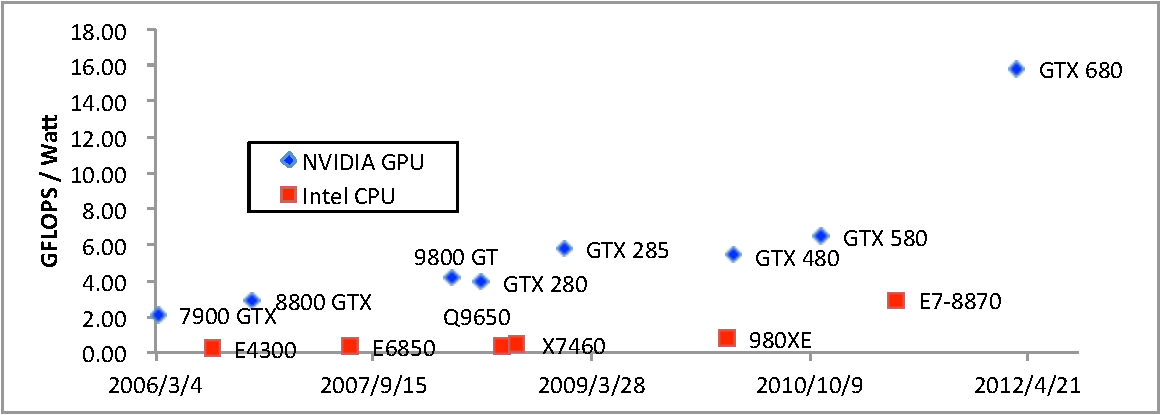
\includegraphics[width=0.46\textwidth]{figures/perf_per_watt.pdf}
 \label{fig:perf_per_watt}
 \caption{Performance-per-watt trends on representative NVIDIA GPUs and
 Intel CPUs.}
\end{figure}

Despite a rapid growth of GPU technology, there has been not much
understanding of power and performance implications of GPU-accelerated
systems.
According to vendor's specifications, the thermal design power (TDP) of
state-of-the-art GPUs is around 200W, while that of today's multicore
CPUs is typically below 100W.
Such a difference in the scale of TDP between CPUs and GPUs prevents
system designers from predicting the power and performance of
GPU-accelerated systems, which makes it difficult, if not impossible, to
optimize their energy savings.
Previous work~\cite{Hong2009,Hong2010,Jiao2010,Lee2011,Nagasaka2010} on
the power and performance analysis of GPU-accelerated systems are based
on either simulation studies or limited hardware functionality.
None of previous work has ever disclosed a fundamental approach to the
power and performance analysis of GPU-accelerated systems.

The contribution of this paper is to provide a power and performance
analysis of GPU-accelerated systems using NVIDIA's \textit{Fermi}
architectures.
Specifically, we identify when to scale the frequency and voltage of
GPUs and CPUs in order to minimize overall system energy.
Our analysis opens up important problems of dynamic voltage and
frequency scaling (DVFS) algorithms for growing GPU-accelerated
systems.
We also provide an open method and tool to scale voltage and frequency
of GPUs.
The black box feature of current GPU drivers and runtimes prevents
researchers from tackling correlative power and performance optimization
problems.
Sharing such a common method and tool with researchers
would further facilitate use of GPUs.

The rest of this paper is organized as follows.
%Section~\ref{sec:background} describes the background and motivation
%behind this work.
Section~\ref{sec:platform} presents our system platform.
Section~\ref{sec:evaluation} provides our evaluation.
Section~\ref{sec:related_work} discusses related work, and this paper
concludes in Section~\ref{sec:conclusion}.

\section{System Platform}
\label{sec:platform}

\begin{table}[!t]
 \caption{Performance levels of GTX 480 (GPU).}
 \vspace{-2.0mm}
 \label{tab:GPU-frequency}
 \footnotesize
 \begin{center}
  \begin{tabular}{|c|c|c|c|}
   \hline
   Clock Domains &Min [MHz]&Low [MHz] & High [MHz]\\
   \hline
   \hline
    Core & 50 & 405 & 700\\
    \hline
    Memory & 135 & 324 & 1848\\
   \hline
  \end{tabular}
  \vspace{-5.0mm}
 \end{center}
\end{table}

\begin{table}[!t]
 \caption{Performance levels of Core i5 2400 (CPU).}
 \small
 \label{tab:CPU-frequency}
 \begin{center}
  \begin{tabular}{|c|c|c|c|}
   \hline
   Platforms&Min [MHz]&Low [MHz]&High [MHz]\\
   \hline
   \hline
   Core i5-2400 &1600& 2700 & 3300.1\\
   \hline
  \end{tabular}
 \end{center}
 \end{table}

We use an NVIDIA GeForce GTX 480 graphics card and Intel Core i5 2400
processor with the Linux kernel 3.3.0.
Table~\ref{tab:GPU-frequency}~and~\ref{tab:CPU-frequency} present their
available performance levels respectively.
To perform the experiment, we use NVIDIA's proprietary
software~\cite{BLOB} and Gdev~\cite{Kato2012} case by case.
NVIDIA's proprietary software does not provide a system interface to
scale the performance level of the GPU.
We hence provide the modified BIOS files for the GPU that force the
binary driver to configure the GPU with the specified performance level
when loaded.
This method enables us to choose any set of the GPU core and memory
clocks, but requires the driver to reload, and the configuration is
static while the driver is running.
On the other hand, Gdev allows the system to change the performance
level of the GPU dynamically at runtime through the Linux ``/proc'' file
system interface.
However, it is available only for the GPU core clock at the moment, and
the GPU memory clock is fixed at 135MHz.
This is limited due to an open-source implementation of Linux, but will
be removed in the future release.

The experimental workload executes the Rodinia benchmark suite
2.0.1~\cite{Che2010} and our original microbenchmark programs of matrix
computation.
All input data for the Rodinia programs use the maximum feasible size,
while the microbenchmark programs vary data size to conduct fine-grained
measurements, all of which are written in CUDA.
We use the NVIDIA CUDA Compiler (NVCC) 4.0~\cite{CUDA40} to compile the
programs.
Both NVIDIA's proprietary software and Gdev receive the same program
binary.

The power and energy consumption of the system is measured by the
YOKOGAWA WT1600 digital power meter.
This instrument obtains the voltage and electric current every $50ms$
from the power plug of the machine.
The power consumption is calculated by multiplying the voltage and
current, while the energy consumption is derived by accumulation of
power consumption.

\section{Evaluation}
\label{sec:evaluation}

\begin{figure}[!t]
\centering
 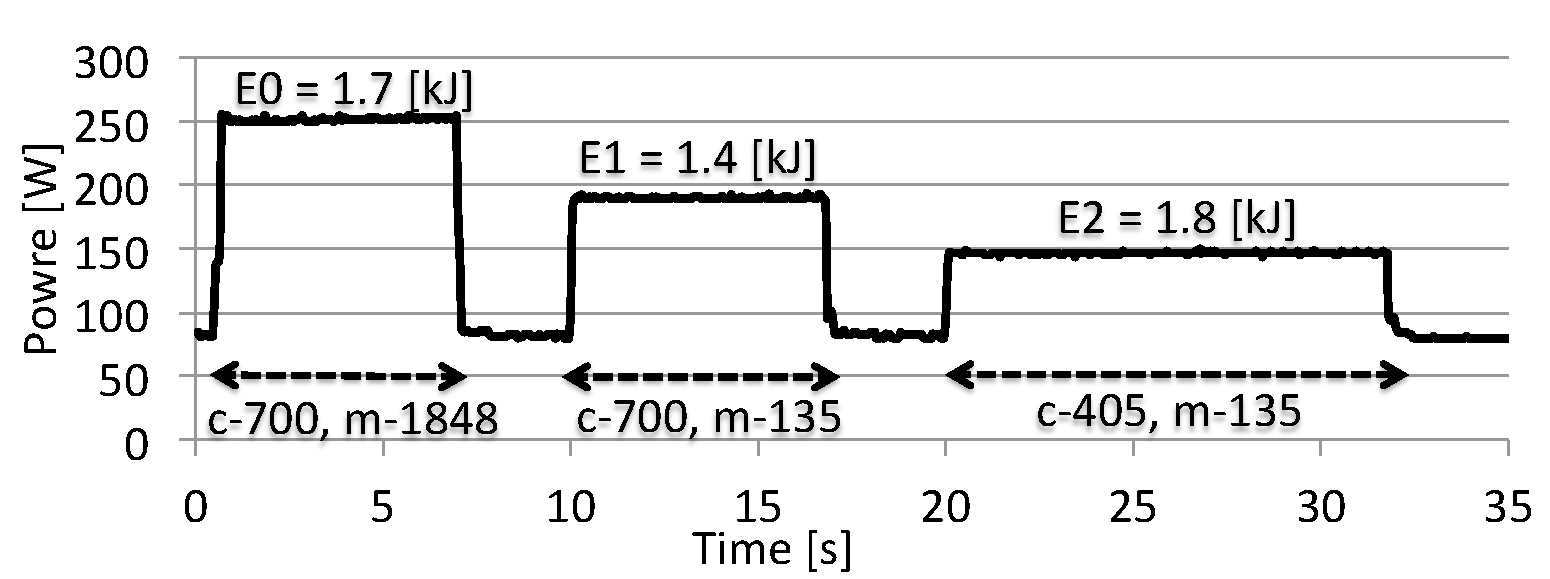
\includegraphics[width=0.45\textwidth]{figures/madd-time-power.pdf}
 \caption{Power consumption and execution time of the $512\times512$
 matrix addition program.}
 \label{fig:madd-time-power}
\end{figure}

We first investigate the impact of GPU core and memory clocks on
GPU-intensive workload executing twenty thousands loops of $512\times512$
matrix addition.
The voltage and frequency of the GPU is changed three times during the
operation, while the CPU is fixed at the minimum level to focus on the
behavior of the GPU.
Figure \ref{fig:madd-time-power} shows the power consumption of the
system in this setup, where ``c-*'' and ``m-*'' stand for the GPU core
and memory clocks respectively, while ``E*'' represents the cummulative
energy consumption of the corresponding duration.
What is learned from this experiment is that energy consumption is
sensitive to the GPU core and memory clocks.
Lowering the memory clock to 135MHz successfully reduces energy
consumption, but the further downscaling of the core clock to 405MHz
counter-increases energy consumption.
This indeed implies DVFS algorithms dominate the power and performance
of GPU-accelerated systems.

We next coordinate the GPU and the CPU using more realistic workload
from the Rodinia benchmark suite.
To simplify the setup, we consider only high (maximum) and low
(minimum) core clocks, meaning that we evaluate four configurations of
(GPU-L, CPU-L), (GPU-H, CPU-L), (GPU-L, CPU-H), and (GPU-H, CPU-H),
where ``*-L'' and ``*-H'' represent the low and high core clocks. 
In an idle state, however, the clocks are always down-scaled to the
minimum level.
We also add another configuration that keeps at the maximum clocks even
though the GPU is idle, in order to see the impact of elementary
coordinated DVFS on GPU-accelerated systems.
Figure~\ref{fig:rodinia-time}~and~\ref{fig:rodinia-energy} respectively
show the execution time and energy consumption of four representative
programs of the Rodinia benchmark suite.
Regarding the execution time, ``all-H'' always takes the shortest
execution time, as it consistently keeps at the maximum performance level.
Other configurations however depend on workload.
For example, the execution time of \texttt{heartwall} -- GPU-intensive
workload -- can be decreased by setting the high GPU clock, whereas that
of \texttt{hotspot} is rather affected by the CPU clock.
The characteristic of energy consumption is more complicated.
For some workload, lowering the clock causes an increase in energy
consumption, as the duration of execution is increased, consuming more
cumulative power consumption.
In other words, GPU-intensive workload should generally use the high GPU
clock so that it completes operation as soon as possible to minimize
energy.
Apparently, ``all-H'' is not a good idea in terms of energy; the clock
should be minimized when the device is not used.
Hence, DVFS is certainly desired but the design of its algorithms is
left an open issue.

\begin{figure}[!t]
\centering
 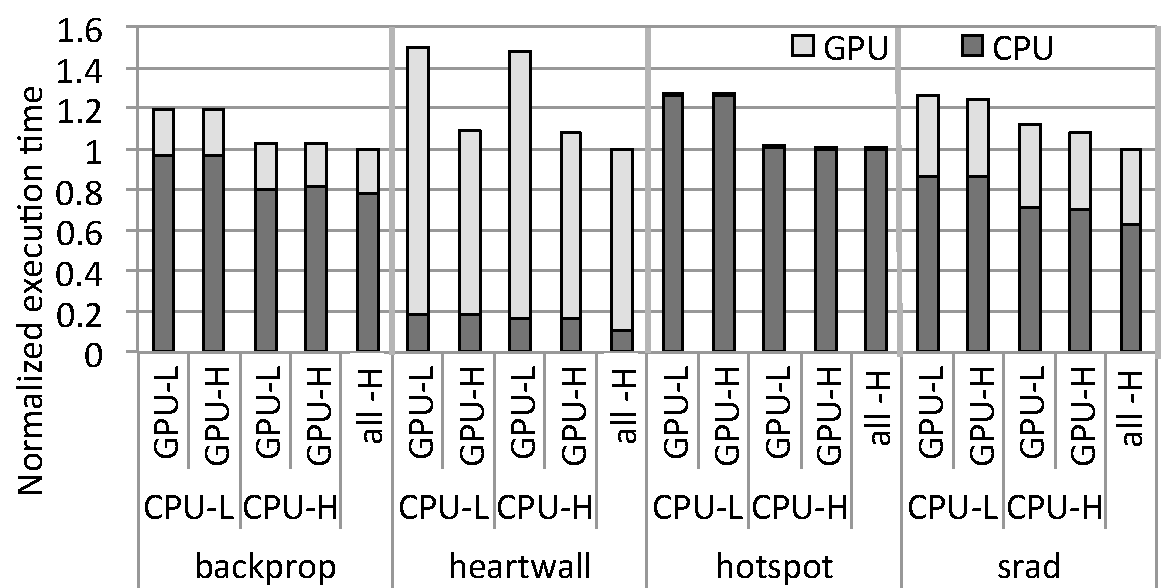
\includegraphics[width=0.45\textwidth]{figures/rodinia-time.pdf}
 \caption{Execution time of the Rodinia programs.}
 \label{fig:rodinia-time}
\end{figure}

\begin{figure}[!t]
\centering
 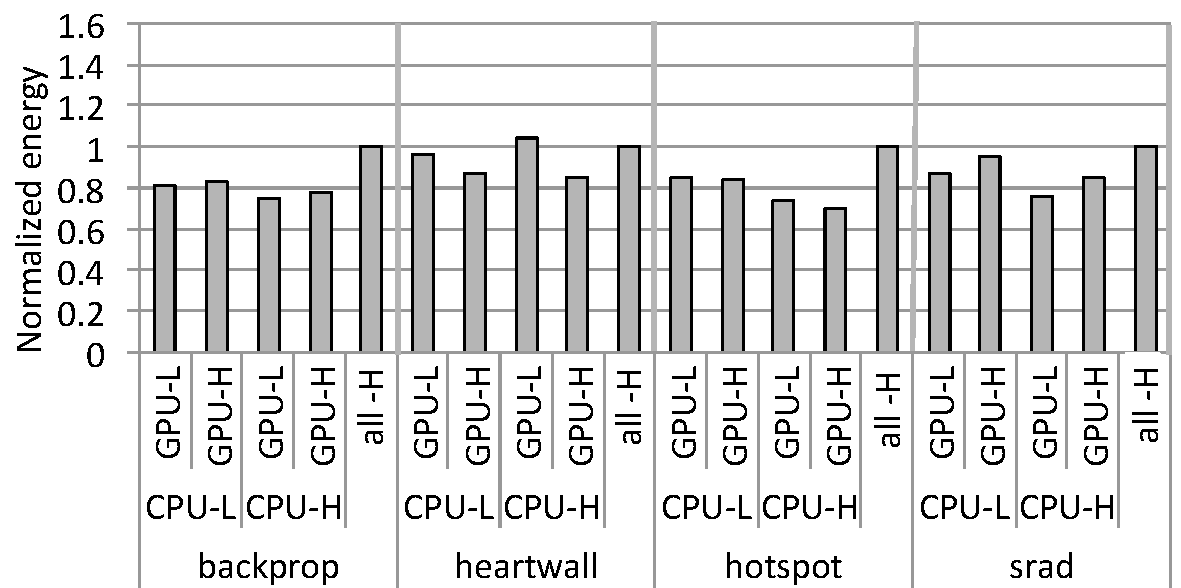
\includegraphics[width=0.45\textwidth]{figures/rodinia-energy.pdf}
 \caption{Energy consumption of the Rodinia programs.}
 \label{fig:rodinia-energy}
\end{figure}

\begin{figure}[!t]
\centering
 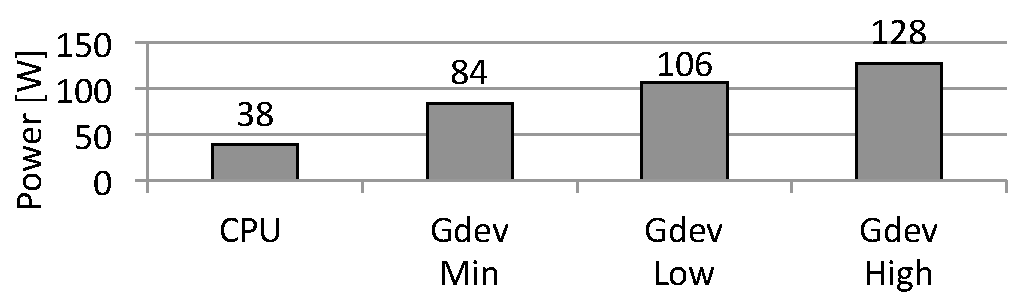
\includegraphics[width=0.45\textwidth]{figures/idol.pdf}
 \caption{Power consumption in an idle state.}
 \label{fig:idle}
\end{figure}

\begin{figure*}[!t]
  \centering
  \subfigure[\texttt{Matrix Addition}]
    {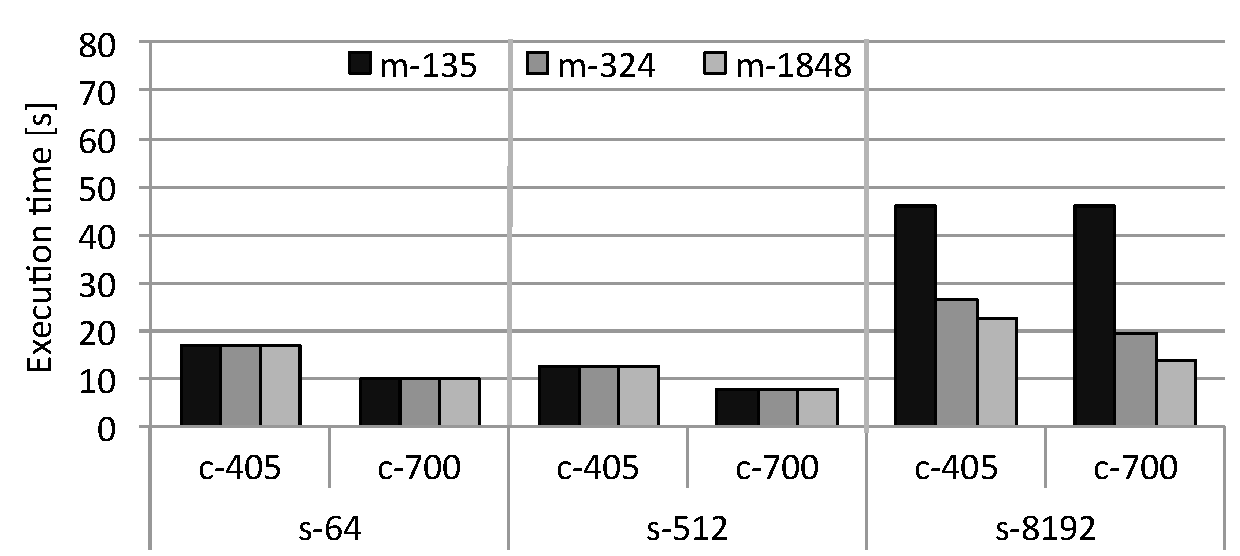
\includegraphics[width=0.45\textwidth]{figures/madd-nvidia-time.pdf}
    \label{madd-time}}
  \subfigure[\texttt{Matrix Multiplication}]
    {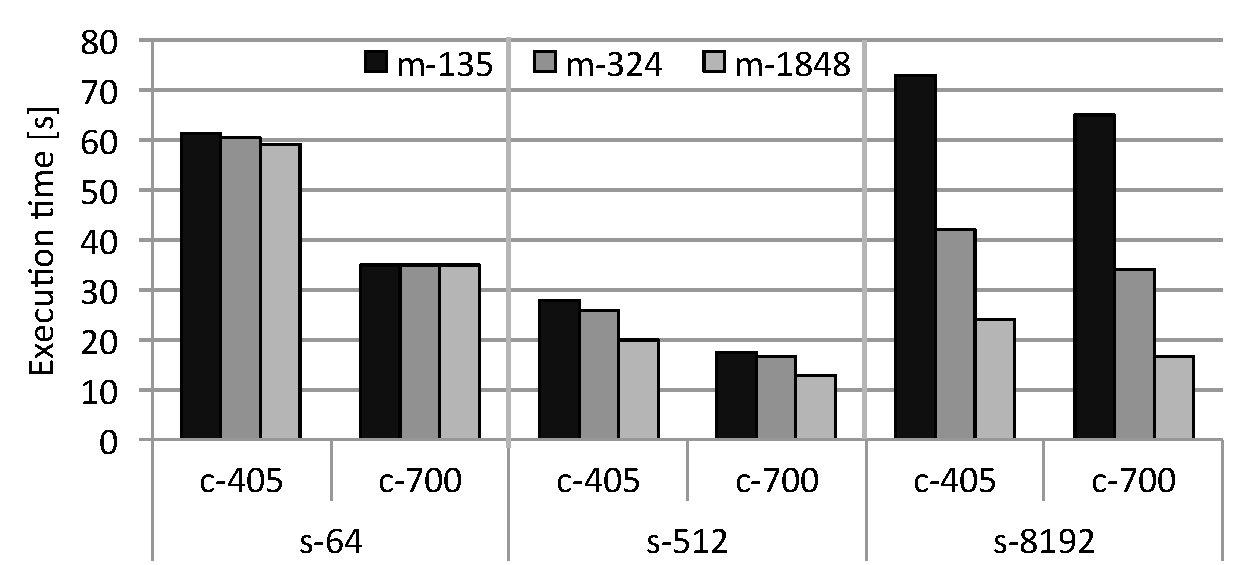
\includegraphics[width=0.45\textwidth]{figures/mmul-nvidia-time.pdf}
    \label{mmul-time}}
  \vspace{-5.0mm}
  \caption{Execution time of the matrix addition and multiplication
 programs.}
  \label{fig:gpu-time}
\end{figure*}

\begin{figure*}[!t]
  \centering
  \subfigure[\texttt{Matrix Addition}]
    {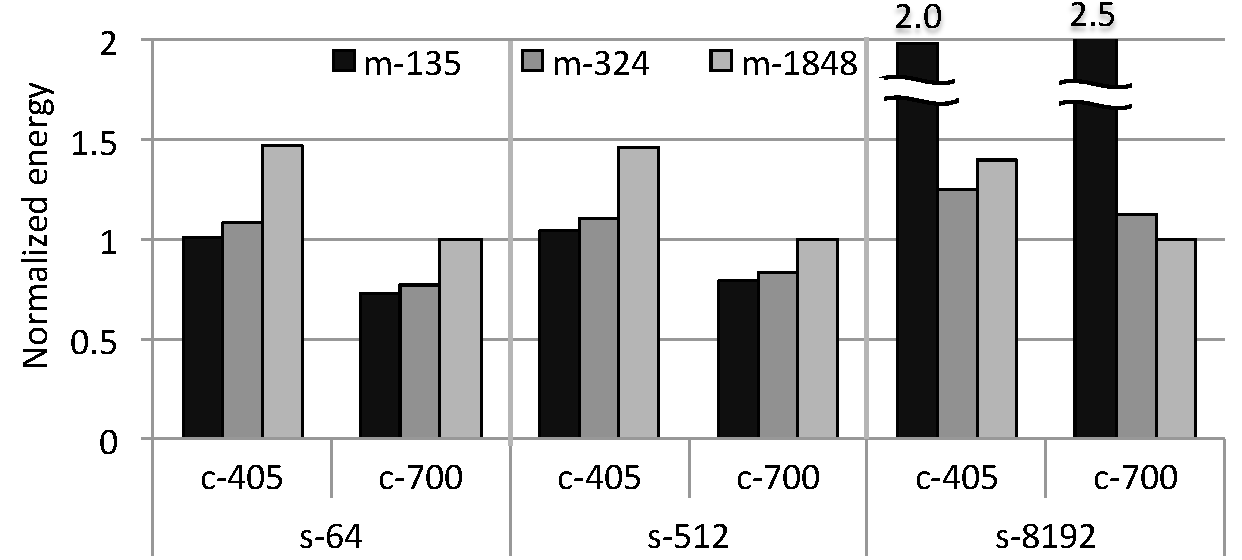
\includegraphics[width=0.45\textwidth]{figures/madd-nvidia-energy.pdf}
    }
  \subfigure[\texttt{Matrix Multiplication}]
    {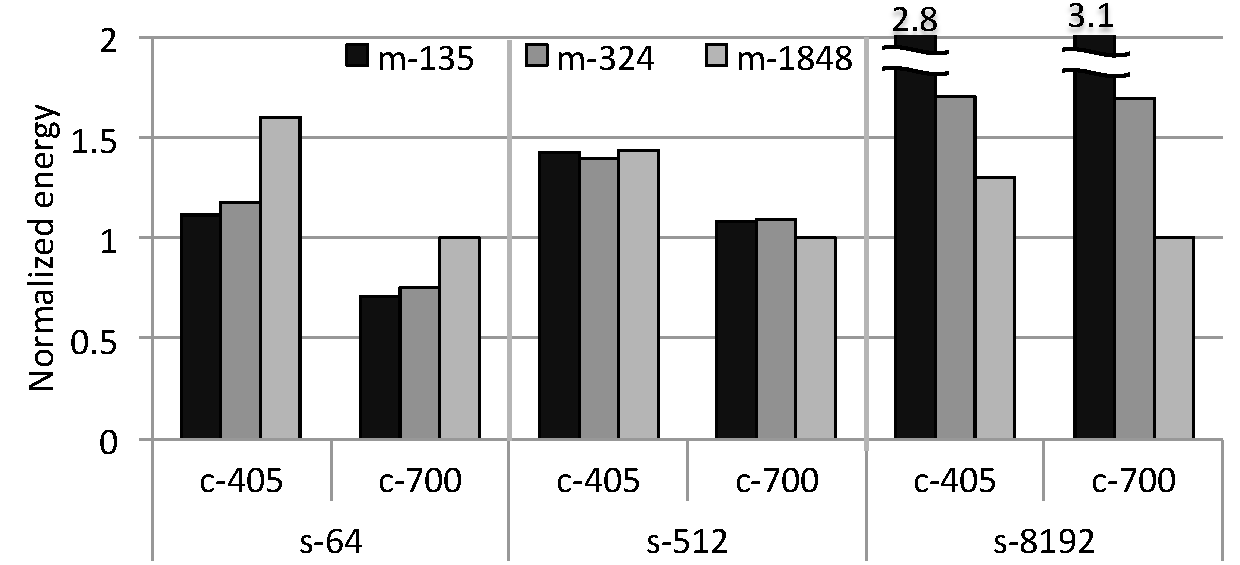
\includegraphics[width=0.45\textwidth]{figures/mmul-nvidia-energy.pdf}
    }
  \vspace{-5.0mm}
  \caption{Energy consumption of the matrix addition and multiplication
 programs.}
  \label{fig:gpu-energy}
\end{figure*}

\begin{figure}[!t]
  \centering
  \subfigure[\texttt{Execution Time}]
    {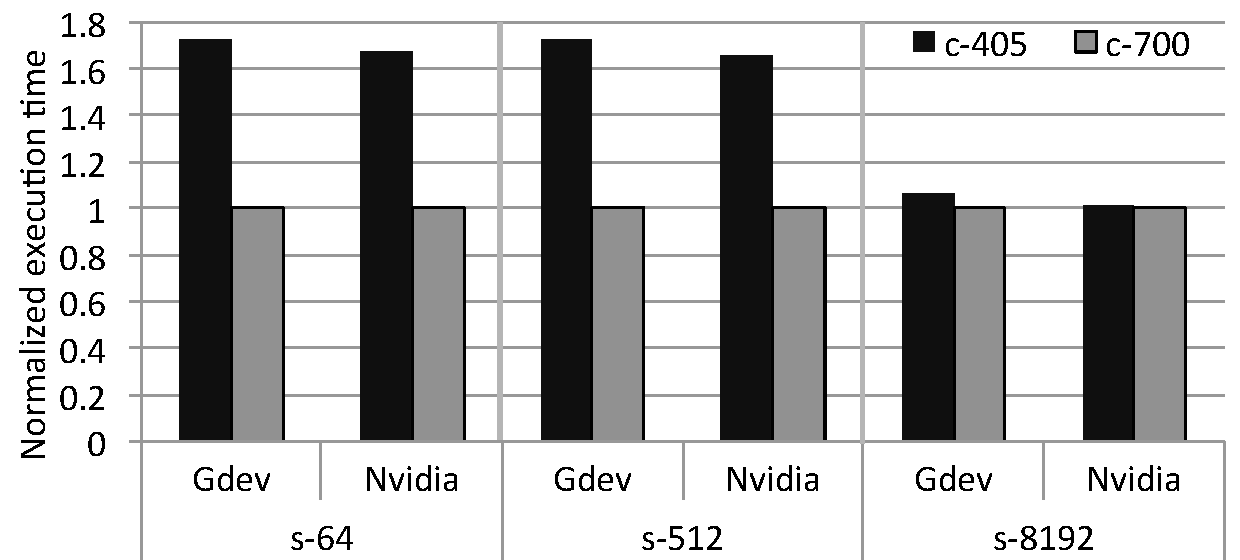
\includegraphics[width=0.45\textwidth]{figures/madd-gdev-nvidia-time.pdf}
    }
  \subfigure[\texttt{Energy Consumption}]
    {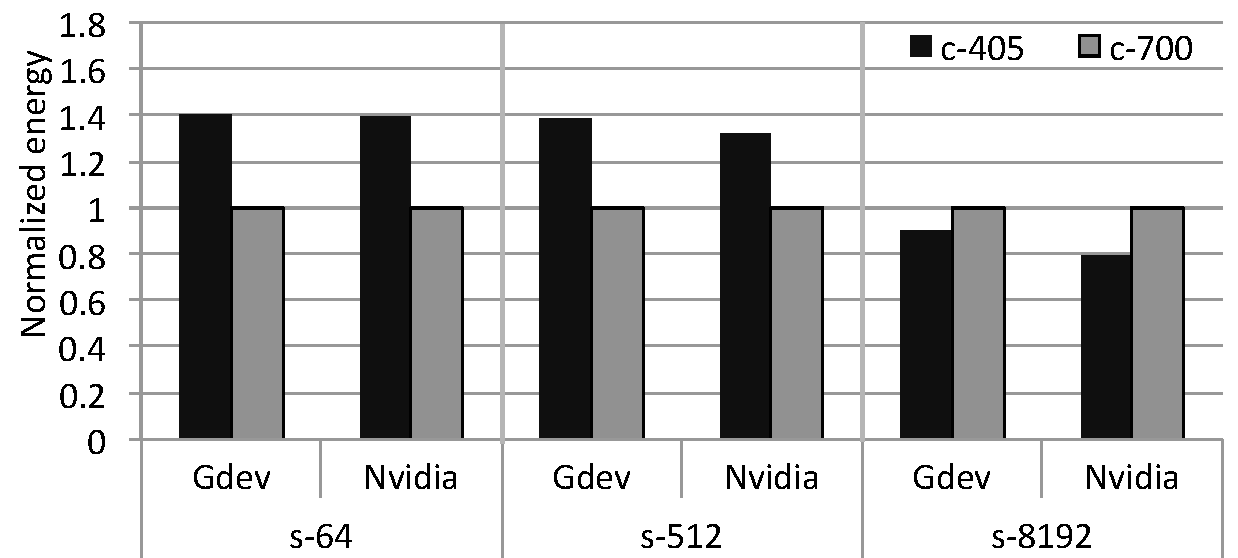
\includegraphics[width=0.45\textwidth]{figures/madd-gdev-nvidia-energy.pdf}
    }
  \vspace{-5.0mm}
  \caption{Comparison of the NVIDIA proprietary and the Gdev open-source
 runtimes and drivers.}
  \label{fig:nvidia-gdev}
\end{figure}

In the above experiments, we have never observed that energy consumption
is reduced by lowering the CPU clock. 
This is because lowering the CPU clock causes the GPU to increase the
duration of an idle state, and there is no power gating support for the
GPU at the moment.
Hence, energy is always wasted when the GPU is idle.
We demonstrate how energy is wasted in an idle state, when (i) the GPU
is not present and (ii) is present with three levels of a set of voltage
and frequency.
Figure~\ref{fig:idle} shows the average power consumption of those four
cases obtained by running the system for 60 seconds.
The CPU consumes no more than 38W on average, whereas the GPU-installed
systems consume a different scale of power depending on the configured
set of voltage and frequency.
This observation encourages the system not to downscale the voltage and
frequency of the CPU, unless the GPU supports power gating to totally
cut off its consuming power.
Another lesson learned from this experiment is that the power
consumption of the GPU is significant even in an idle state, meaning
that DVFS is strongly desired for the GPU with whatever overhead it has
to pay for changing the performance level.

The preceding evaluation indicates that the CPU is a weak factor for
energy savings of GPU-accelerated systems.
Henceforth, we restrict our attention to the GPU.
According to the traditional power modeling~\cite{Hsu2001}, lowering the
core clock is often effective for memory-intensive workload.
Our next evaluation verifies if the same is true for the GPU.
We use matrix addition and multiplication programs with varied sizes of
data.
A small size of data reduces memory accesses, while a large size of data
makes the workload memory-intensive.
Figure~\ref{fig:gpu-time}~and~\ref{fig:gpu-energy} show the execution
time and energy consumption of those matrix computations, where ``s-*''
represents the number of matrix row/column.
A difference between ``s-64'' and ``s-8192'' explains that memory-clock
scaling is more effective for such computations that use a smaller size
of data.
This is because the execution time of such computations is not
affected by lowering the memory clock.
Another observation is that energy cannot be saved by lowering the core
clock, because these matrix computations are consistently
compute-intensive.
If the core clock is downscaled, their execution time is highly
increased, which results in an increase in cumulative power
consumption.

Seen from the above experiments, system energy could be reduced
by about 28\% retaining a decrease in performance within 1\%.
These experimental results encourage that DVFS algorithms for
GPU-accelerated systems should be weighted on the GPU rather the CPU,
though their energy optimization is very challenging, given many factors
of design knobs including CPU/GPU, core/memory, and workload
characteristics.

Finally, we compare NVIDIA's proprietary software and Gdev.
This is an important and practical investigation in that NVIDIA's
proprietary software does not expose a system interface to change
the voltage and frequency of the GPU dynamically at runtime, and hence
the development of DVFS algorithms in future work will inevitably depend
on Gdev.
The basic performance of Gdev is competitive to NVIDIA's proprietary
software~\cite{Kato2012}, but we have to evince that Gdev is also
reliable for power management.
The test program exploits matrix addition with varied sizes of data.
Figure~\ref{fig:nvidia-gdev} shows the execution time and energy
consumption of the matrix addition programs using different scales of
GPU core clocks, where the GPU memory clock is fixed at 135MHz.
In this experiment, ``s-8192'' benefits from lowering the core clock,
because the workload is memory-bound due to a large size of matrix, and
the execution time is not much affected by the core clock, while every
is effectively saved.
The most remarkable observation is that NVIDIA's proprietary software
and Gdev exhibit almost the same results on the execution time and energy
consumption.
This implies that the result of our on-going research using Gdev could
be easily propagated to the real product, once energy management
interfaces are employed by vendor's software.

\section{Related Work} 
\label{sec:related_work}

Nagasaka \textit{et al.} conjectured energy consumption of GPUs based on
the hardware performance counter~\cite{Nagasaka2010}.
This performance counter, however, is not adequate in that power
consumption rises even in an idle state when voltage and frequency are
scaled, though the performance counter does not change in an idle
state.
Hence, this approach would require an additional model to precisely
analyze the power consumption of the GPU.

Hong \textit{et al.} studied energy savings of GPUs, assuming power
gating available to limit the number of active
cores~\cite{Hong2009,Hong2010}.
In particular, they analyze PTX code to model the power and performance
of GPUs based on the number of instructions and memory accesses.
Unfortunately, none of the current GPU architectures yet supports power
gating, which limited their contribution to simulation studies.
Therefore, it is questionable if the presented power and performance
model is applicable to the real-world, and GPU power gating is also not
a realistic assumption at the moment.
Nonetheless, we consider that an offline PTX analysis for power and
performance prediction is a useful approach to the design of DVFS
algorithms.
What lacks in this approach, however, is a runtime analysis for input
data.
In this paper, we have analyzed the power and performance
characteristics depending on the size of input data. 

Lee \textit{et al.} presented a method to apply DVFS algorithms to the
GPU.
They particularly aimed at maximizing performance under the given power
constraint~\cite{Lee2011}.
A strong limitation of their work, however, is that the evaluation of
power consumption is based on a conceptual model but not on real-world
hardware.
They also failed to discuss how to determine the voltage and frequency.
In this paper, we have rather explored how to minimize the energy
consumption of GPU-accelerated systems using the cutting-edge real-world
hardware.

Jiao \textit{et al.} evaluated the power and performance of an old
NVIDIA GTX~280 GPU~\cite{Jiao2010}.
They examined compute-intensive and memory-intensive programs.
According to their analysis, energy consumption could often be reduced
by lowering the core clock when workload is memory-intensive.
This is exactly the same as what we have identified for an NVIDIA's
GTX~480 GPU.
Therefore, we conjecture that this observation and knowledge could be
applied to future GPU architectures as well.
In addition, we have disclosed that energy consumption could also be
reduced by scaling the memory clock.
This opens up a new insight into DVFS algorithms for GPU-accelerated
systems.

Ying \textit{et al.} analyzed the power and performance of an AMD
HD~5870 GPU using a random forest method with the profile
counter~\cite{ying2011}.
They revealed that activating a fewer number of ALUs reduces power
consumption.
However, this approach incurs an increase in execution time, and does
not successfully reduce energy consumption.
This is attributed to the fact that they use only software management.
Meanwhile, we have demonstrated that energy can be reduced by scaling
the voltate and frequency of the GPU.

\section{Conclusion and Future Work}
\label{sec:conclusion}

We have presented a power and performance analysis of GPU-accelerated
systems based on the NVIDIA Fermi architecture.
Our findings include that the CPU is a weak factor for energy savings of
GPU-accelerated systems unless power gating is suppoted by the GPU.
In contrast, voltage and frequency scaling of the GPU is significant to
reduce energy consumption.
Our experimental results demonstrated that system energy could be reduced
by about 28\% retaining a decrease in performance within 1\%, if the
performance level of the GPU can be scaled effectively.

In future work, we plan to develop DVFS algorithms for GPU-accelerated
systems, using the characteristic identified in this paper.
We basically consider such an approach that controls the GPU core clock
for memory-intensive workload while controls the GPU memory clock for
compute-intensive workload.
To this end, we integrate PTX code analysis~\cite{Hong2009,Hong2010}
into DVFS algorithms so that energy optimization can be provided at
runtime.
We also consider a further dynamic scheme that scales the performance
level of the GPU during the execution of GPU code, whereas we restricted
a scaling point at the boundary of GPU code in this paper.

\setlength{\bibspacing}{\baselineskip}
{\scriptsize \bibliographystyle{acm}
\bibliography{refer}}

% Use the following at camera-ready time to suppress page numbers.  Comment it
% out when you first submit the paper for review.
\thispagestyle{empty}
\end{document}
